\chapter{Diseño y arquitectura del sistema}

\section{Estructura general}

El código del trabajo y todo lo que abarca se encuentra almacenando en \href{https://github.com/orgs/vieites-tfg/repositories?type=source}{GitHub}. Se han creado los repositorios necesarios en una misma organización de GitHub.

Entre los repositorios creados se pueden encontrar:

\begin{itemize}
  \item \texttt{zoo}.

    Este es el repositorio principal. Se trata de un \textit{monorepo}, en el que se encuentra implementado todo el código necesario para la realización del trabajo. Dentro del repositorio se encuentran:
    \begin{itemize}
      \item La aplicación de prueba sobre la que se apoya el proyecto, y que da nombre al repositorio, debido a que se trata de una aplicación de gestión de un zoo.
      \item Los módulos de Dagger para realizar los ciclos de CI y CD.
      \item Otros archivos, como \textit{scripts} y archivos de configuración.
    \end{itemize}

  \item \texttt{helm-repository}.

    Este repositorio alberga las Charts de Helm que definen la estructura necesaria para desplegar la aplicación de prueba.

  \item \texttt{state}.

    Se trata del repositorio en el que se almacenan los valores que poblarán los recursos de Kubernetes, dependiendo del entorno en los que se despliegue la aplicación. Además, en este repositorio también existe una rama de despliegue, de la cual ArgoCD lee los manifiestos de los recursos que debe desplegar para cada uno de los entornos.
\end{itemize}

En la figura~\ref{fig:ghorg} se muestra un diagrama de la disposición de los repositorios y la relación entre ellos.

\begin{figure}
  \centerline{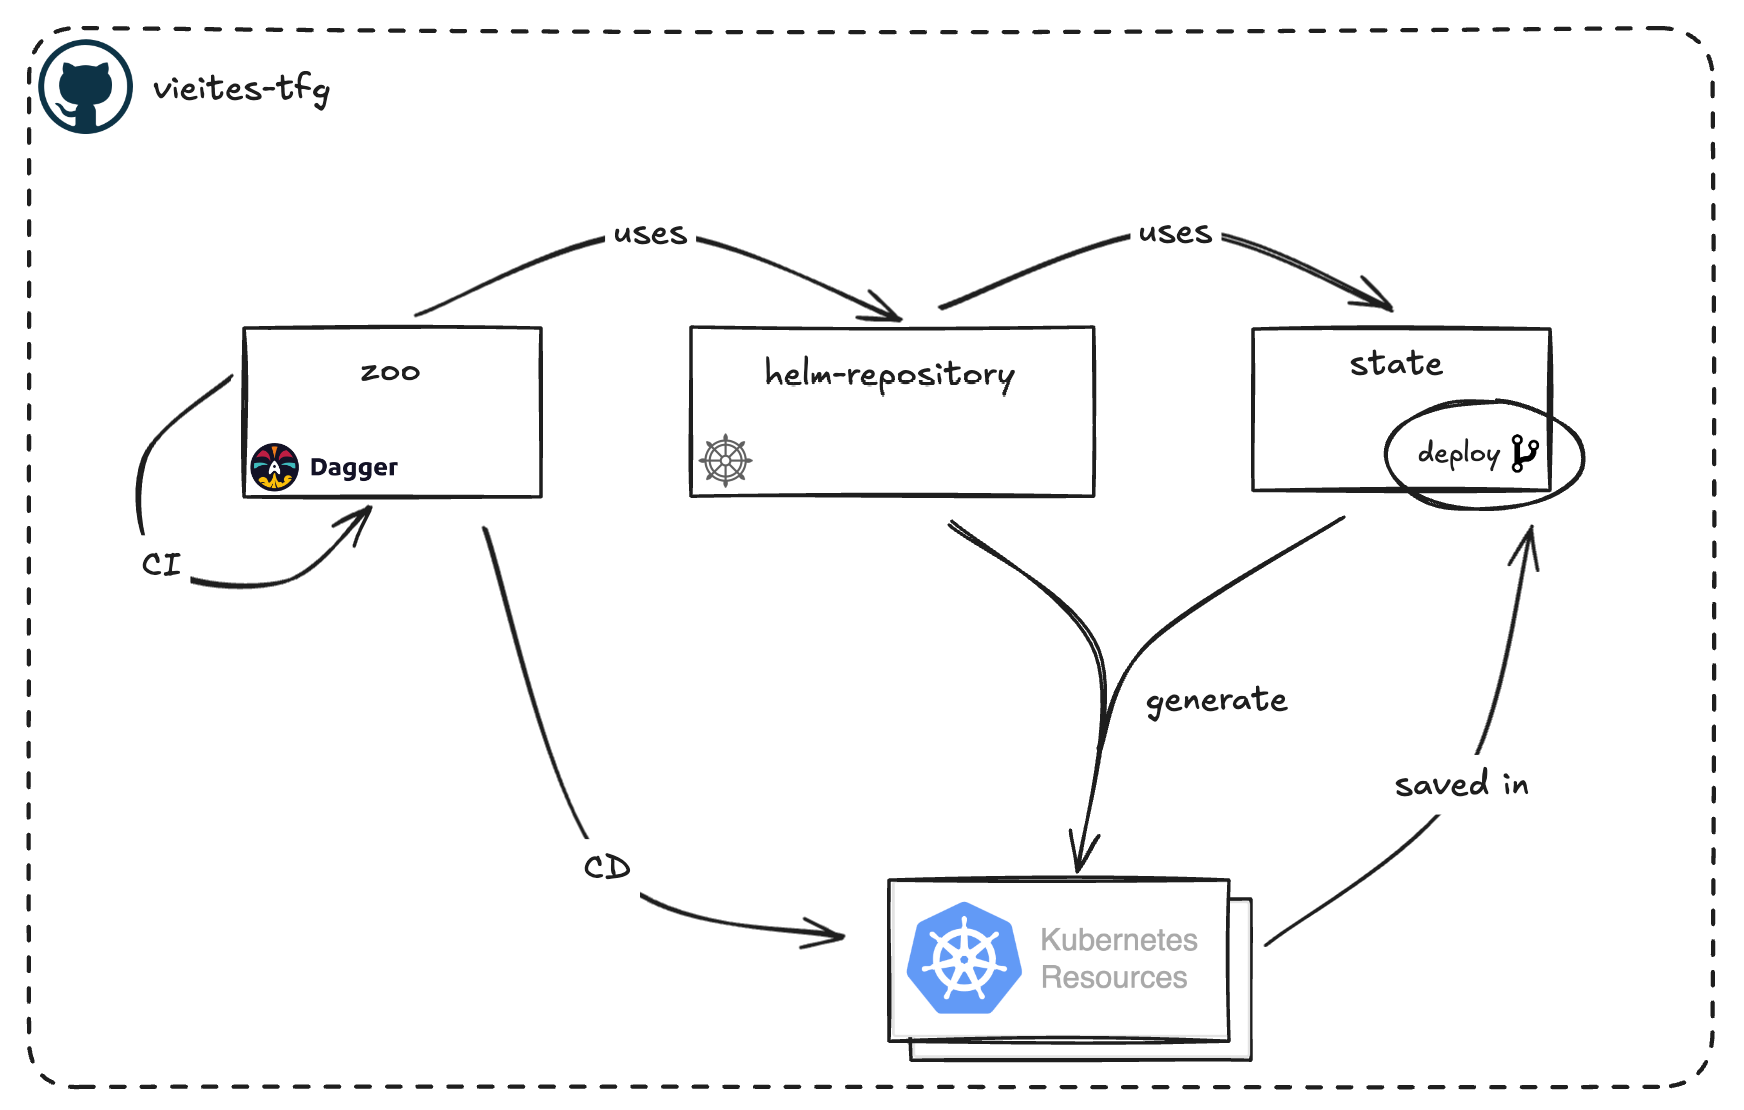
\includegraphics[width=15cm]{figuras/vieites-tfg}}
  \caption{Diagrama del la organización de GitHub}
  \label{fig:ghorg}
\end{figure}

\section*{zoo}

Como se ha comentado anteriormente, el repositorio \texttt{zoo} está estructurado como un \textit{monorepo}. Un \textit{monorepo} es un repositorio con diferentes proyectos, los cuales se encuentran interrelacionados de una manera bien definida. A lo largo de esta sección se justifica la elección de este tipo de estructura, a la vez que se explica cómo están implementados las diferentes piezas de software.

\subsection*{Aplicación de prueba}

La primera razón para escoger este tipo de estructura es el hecho de querer crear una aplicación relativamente pequeña, una página web que consta de un \textit{frontend} y un \textit{backend} (se hará referencia a estos como ``paquetes'' a partir de ahora). Por lo tanto, se hace más sencillo gestionar estos dos paquetes si viven juntos en un único repositorio.

Otra ventaja de utilizar un \textit{monorepo} tiene que ver con el software utilizado para crear los paquetes de la aplicación de prueba. Ambos se implementan utilizando Node.js, en lenguaje Typescript\cite{ts}. Los paquetes tienen dependencias propias, y se puede dar el caso de que ambos utilicen una o varias dependencias iguales. Usar un \textit{monorepo} permite tener esas dependencias en un mismo lugar, evitando su duplicado. Con esto se consigue reducir el tiempo de construcción de los paquetes.

Sin embargo, es necesaria una herramienta que permita manejar los paquetes de manera independiente. Alguno de los motivos para tener esta preferencia pueden ser: que haya dos equipos de desarrolladores, uno para cada paquete; o que se quiera publicar versiones, hacer tests, u otro tipo de tarea sobre cada paquete por separado. La herramienta que se utiliza en este trabajo se llama Lerna\cite{lerna}. Este software está específicamente diseñado para gestionar \textit{monorepos} de proyectos de Node.js. Entre las ventajas que proporciona se encuentran:

\begin{itemize}
  \item Gestión de tareas locales.
  \item Cacheo local de salidas de comandos, con posibilidad de dicha caché sea compartida entre entornos, por ejemplo, con agentes de CI.
  \item Detección de paquetes afectados por cambios en el código.
  \item Análisis de la estructura del proyecto.
\end{itemize}

Por los beneficios anteriormente comentados, y más, es por lo que se ha elegido esta herramienta para gestionar el \textit{monorepo}.

En cuanto a las tecnologías que se utilizan en la aplicación, ya se ha mencionado Typescript como lenguaje principal. Este lenguaje permite tener un sistema tipado, lo cual puede ser útil para detectar muchos errores comunes mediante el análisis estático en tiempo de construcción. Esto reduce las posibilidades de errores en tiempo de ejecución.

El \textit{backend} está completamente desarrollado utilizando dicho lenguaje. Su funcionalidad es proporcionar una API REST que el \textit{frontend} pueda utilizar para realizar cambios en la base de datos. Se usa MongoDB\cite{mongodb} como base de datos debido a que es fácil de gestionar y porque solo se almacena información sobre animales, sin ningún tipo de relación entre ellos, en una única tabla o documento.

El \textit{frontend} se ha implementado utilizando Vue.js\cite{vue}, un \textit{framework} que permite construir interfaces web mediante componentes reactivos. Se ha escogido este frente a otras opciones debido a su facilidad de uso sin conocimiento previo. Tiene una API intuitiva, por lo que no tiene una gran curva de apendizaje. Además, el propio \textit{framework} está construido utilizando Typescript, por lo que tiene compatibilidad de primera clase con este lenguaje.

\subsection*{Módulos de Dagger}

Se integran también en el repositorio los módulos de Dagger de CI y de CD. Estos módulos se incluyen en el \textit{monorepo} para facilitar la referencia a los paquetes que constituyen la aplicación de prueba. Además, tiene sentido que vivan en el mismo lugar una aplicación y las herramientas que permiten su evolución, como son cualquier tipo de software que realice las funciones de CI y de CD.

Ambos módulos se realizan utilizando el SDK del lenguaje Go que proporciona Dagger. Se ha escogido este lenguaje debido al conocimiento previo que ya se tenía de este. Además, es el lenguaje en el que está implementado el propio Dagger.

Uno de los módulos se encarga del ciclo de CI, es decir, de realizar los tests de la aplicación, del \textit{linting} o análisis del código en sí, y dela publicación de imágenes de Docker y paquetes NPM. Está organizado de manera que se pueden gestionar cada uno de los paquetes de la aplicación de manera independiente. Esto también es posible gracias al uso de Lerna, que ya se ha comentado anteriormente.

El segundo de los módulos, el de CD, realiza la tarea de publicación de los recursos de Kubernetes, los cuales son posteriormente obtenidos por ArgoCD para su despliegue completo. Esto se consigue haciendo uso de los repositorios \texttt{helm-repository} y \texttt{state}, en los cuales se almacenan las Charts de Helm y los valores que pueblan dichas Charts, respectivamente.

Se detalla más profundamente su implementación en el capítulo \ref{chap:dagger}.

\subsection*{Creación y configuración de los \textit{clusters}}
\label{subsec:clusters}

La fase final del ciclo de una aplicación es el despliegue. En este trabajo se levantan tres \textit{clusters} de KinD de manera local. Estos son los lugares en los que se despliega la aplicación. Generalmente se tienen diferentes \textit{clusters} con el fin de probar la aplicación en entornos distintos antes de desplegarla en el principal, que sería el de producción. El hecho de crearlos todos localmente hace que sean más sencillas las pruebas relacionadas con el despliegue. En equipos de desarrollo reales, los entornos de producción se encuentran en la nube. Sin embargo, sí que se pueden llegar a tener entornos locales para realizar pruebas de la aplicación.

Los \textit{clusters} se crean con el \textit{script} que se muestra en el Linting \ref{lst:create-clusters}. Se han puesto comentarios en vez de código algunas partes para reducir su tamaño, a modo de pseudocódigo. Estos son los pasos que se siguen para crear cada uno de los \textit{clusters}:

\begin{enumerate}
  \item Se indica el banner que va a tener cada uno de los \textit{clusters} (líneas 5-12).
  \item Se indica el contexto actual (línea 14), lo cual identifica cada \textit{cluster}. Esto es necesario a la hora de ejecutar comandos con \texttt{kubectl}, para asegurarse de que se está ejecutando cada comando sobre el \textit{cluster} que se precisa.
  \item Se crea el \textit{cluster} con su configuración específica.
\end{enumerate}

\begin{lstlisting}[language=bash,label=lst:create-clusters]{Script de creación de los clusters}
# Variables globales
# ---

for ENV in "${ENVS[@]}"; do
  case "${ENV}" in
    dev)
      BANNER_TEXT="We are in DEV";;
    # ... otros entornos
  esac

  CONTEXT="kind-${ENV}"

  echo "--- Creating cluster '${ENV}' ---"
  kind create cluster --config "${CLUSTER_DIR}/kind_${ENV}.yaml"

  echo "--- Installing Ingress Controller in cluster '${ENV}' ---"
  kubectl apply -f "${INGRESS_MANIFEST}" --context "${CONTEXT}"
  kubectl wait --namespace ingress-nginx \
    --for=condition=ready pod \
    --selector=app.kubernetes.io/component=controller \
    --timeout=120s \
    --context "${CONTEXT}"

  kubectl create namespace argocd || true

  echo "--- Applying SOPS AGE Key for ArgoCD ---"
  cat "${SOPS_DIR}/age.agekey" |
    kubectl create secret generic sops-age -n argocd --context ${CONTEXT} \
    --from-file=keys.txt=/dev/stdin

  echo "--- Installing ArgoCD in cluster '${ENV}' ---"
  helm repo add argo https://argoproj.github.io/argo-helm
  helm repo update
  helm install argocd argo/argo-cd \
    -n argocd \
    -f argo/values.yaml \
    --wait \
    --version 6.11.1 \
    --kube-context "${CONTEXT}"

  kubectl wait --for=condition=Available deployment --all \
    -n argocd --context "${CONTEXT}" --timeout=5m

  echo "--- Applying ArgoCD application for '${ENV}' ---"
  kubectl apply -f "${ARGO_DIR}/argo_${ENV}.yaml" --context "${CONTEXT}"
  kubectl wait --for=condition=Ready pod -l app.kubernetes.io/name=argocd-server \
    -n argocd --context "${CONTEXT}" --timeout=5m

  echo "--- Applying ArgoCD UI banner for '${ENV}' ---"
  kubectl patch configmap argocd-cm -n argocd --context "${CONTEXT}" --type merge \
    -p "{\"data\":{\"ui.bannercontent\":\"${BANNER_TEXT}\"}}"

  echo "--- Cluster '${ENV}' setup complete ---"
  pass=$(kubectl -n argocd get secret argocd-initial-admin-secret \
    -o jsonpath="{.data.password}" | base64 -d)

  current_pass="${ENV} password: ${pass}\n"
  printf "${current_pass}"
  PASSWORDS+="${current_pass}"
done

echo "--- All environments created successfully! ---"
printf "${PASSWORDS}"
\end{lstlisting}

\begin{lstlisting}[language=helm,label=lst:conf-cluster]{Configuracion del cluster de dev}
kind: Cluster
apiVersion: kind.x-k8s.io/v1alpha4
name: dev
networking:
  apiServerPort: 6443
nodes:
- role: control-plane
  kubeadmConfigPatches:
  - |
    kind: InitConfiguration
    nodeRegistration:
      kubeletExtraArgs:
        node-labels: "ingress-ready=true"
  extraPortMappings:
  - containerPort: 80
    hostPort: 8080
    protocol: TCP
  - containerPort: 443
    hostPort: 8443
    protocol: TCP
\end{lstlisting}

Los \textit{clusters} que se utilizan son los siguientes:

\begin{itemize}
  \item \texttt{dev}.

    Se trata del \textit{cluster} de desarrollo. En este se despliega la aplicación en el momento en el que se añade una nueva funcionalidad, ya sea en el \textit{frontend} o en el \textit{backend}. Esto implica, en términos de GitHub:

    \begin{enumerate}
      \item Crear una \textit{Pull Request} (PR) en la que se implementa la nueva funcionalidad. Esta debe ser siempre lo más reducida posible, cumpliendo con la filosofía de CI. Esto implica que la intención del equipo de desarrollo debe ser desplegar nuevas funcionalidades o correcciones de errores en producción en el menor tiempo posible. Se puede conseguir esto planeando PRs cortas en cuanto a tiempo de desarrollo, evitando que el equipo tenga demasiado trabajo en progreso y asignando los recursos necesarios para que cada PR se lleve a cabo lo más rápidamente\cite{linear}.
      \item Implementar la funcionalidad o realizar la corrección pertinente. A medida que se implementa, se puede, y es una buena práctica, ejecutar localmente el ciclo de CI para asegurarnos de que se pasan las pruebas y el \textit{linting} del código. Esta es una de las ventajas principales de utilizar Dagger. El desarrollador puede comprobar de manera local si el código actualizado es capaz de pasar el \textit{pipeline} de CI, lo cual evita tener errores inesperados a la hora de integrar el código en la rama principal.
      \item Revisar que la tarea que correspondía hacer en dicha PR se ha realizado correctamente.
      \item Integrar la funcionalidad o corrección en la rama principal del repositorio.
    \end{enumerate}

    Tras haber terminado todos los pasos anteriores, se ejecuta un \textit{workflow} de GitHub que realiza todo el ciclo de CI y CD, independientemente del entorno en el que se vaya a desplegar. El workflow es el que se ve en el Linting \ref{lst:workflowcicd}. En este se realizan los siguientes pasos:

    \begin{enumerate}
      \item Se clonan los repositorios necesarios (líneas 12-15).
      \item Se instala Dagger (líneas 17-18).
      \item Se determina el entorno y la \textit{tag} que se le pondrá a la imagen de Docker de los paquetes de la aplicación (\textit{backend} y \textit{frontend}) (líneas 20-29). Esta \textit{tag} es diferente para cada entorno. En el entorno de \texttt{dev} se trata de los ocho primeros caracteres del último \textit{commit} que se ha realizado. De esta manera se sabe a ciencia cierta el código que conforma la aplicación en dicha imagen, y facilita la detección de errores. El entorno es \texttt{dev} siempre que el evento que haya disparado el \textit{workflow} sea un \textit{push} de la PR a la rama principal, en este caso \texttt{main}.
      \item Se recrean los archivos necesarios con las variables almacenadas en GitHub (líneas 31-39). Se proporcionan estos archivos y datos en los manuales de usuario
        \begin{bclogo}[logo=\bcattention]{Important!}
          CITAR MANUALES DE USUARIO
        \end{bclogo}
        para su testeo en local.
      \item Se ejecuta el ciclo de CI para ambos paquetes de la aplicación y se publica cada una de las imágenes, indicando la \textit{tag} que se ha determinado previamente (líneas 51-57). Además, es necesario actualizar los valores de las \textit{tags} en el repositorio de estado, el cual tiene un campo específico para indicar este dato (líneas 45-49).
        \begin{bclogo}[logo=\bcattention]{Important!}
          CITAR APARTADO EN EL QUE SE HABLA DE STATE
        \end{bclogo}
      \item Se ejecuta el ciclo de CD, aportando los parámetros necesarios, entre los que se encuentran los archivos que se han construido previamente (líneas 59-69).
    \end{enumerate}

    Finalmente, la instancia de ArgoCD instalada en el entorno se sincroniza con el repositorio, obtiene los recursos de Kubernetes que se han almacenado en este y despliega la aplicación.

\end{itemize}


\begin{lstlisting}[language=workflows,label=lst:workflowcicd]{Workflow de CI/CD}
on:
  push:
    branches: [ main ]
  release:
    types: [ published ]
  workflow_dispatch:

jobs:
  cicd:
    runs-on: ubuntu-24.04
    steps:
      - % Clona el repositorio "zoo" en la ruta "/zoo"

      - % Clona el repositorio "state" en la ruta "/state"
        % utilizando el token STATE_REPO

      - name: Install Dagger
        uses: dagger/dagger-for-github@8.0.0

      - name: Determine environment
        id: env_tag
        run: |
          % Determina el entorno en el que se despliega, teniendo
          % en cuenta el *trigger* que ha lanzado el workflow:
          %   - *push*    -> main
          %   - *release* -> *release* o *pre-release*

          echo "environment=${envi}" >> "$GITHUB_OUTPUT"
          echo "tag=${tag}" >> "$GITHUB_OUTPUT"

      - name: Recreate needed files
        run: |
          % Recrea el archivo .env para tenerlo disponible en
          % "zoo"
          echo "CR_PAT=${{ secrets.CR_PAT }}" >> ./.env
          % .... se incluyen todas las variables

          % Almacena la clave privada de "age"
          % Crea el archivo de configuracion de SOPS

      - name: Run Dagger CI module
        run: |
          tag=${{ steps.env_tag.outputs.tag }} 

          update_state () {
            % Actualiza el valor en "state" de la *tag* de la
            % imagen para que se despliegue la que se acaba de
            % publicar
          }

          dagger call --sec-env=file://.env backend \
              publish-image --tag "${tag}"
          update_state "zoo-backend" "${tag}"

          dagger call --sec-env=file://.env frontend \
              publish-image --tag "${tag}"
          update_state "zoo-frontend" "${tag}"

      - name: Run Dagger CD module
        run: |
          dagger call -m "./dagger/cd" \
            --socket=/var/run/docker.sock \
            --kind-svc=tcp://localhost:3000 \
            --config-file=file://cluster/kind_local.yaml \
            deploy \
            --sec-env=file://.env \
            --env=${{ steps.env_tag.outputs.environment }} \
            --age-key=file://sops/age.agekey \
            --sops-config=file://sops/.sops.yaml
\end{lstlisting}

% Además, también se encuentran en este repositorio los módulos de Dagger de CI y de CD, y los \textit{scripts} y archivos de configuración necesarios para lanzar en local los \textit{clusters} de KinD que representan cada uno de los entornos en los que se despliega la aplicación. El hecho de que todo lo anterior se encuentre en un mismo repositorio hace mucho más sencilla su gestión.

% Debe describirse como se realiza o Sistema, a división deste en diferentes compoñentes e a comunicación entre eles. Así mesmo, determinarase o equipamento hardware e software necesario, xustificando a súa elección no caso de que non fose un requisito previo. Debe achegarse a un nivel suficiente de detalle que permita comprender a totalidade da estrutura do produto desenvolvido, utilizando no posible representacións gráficas.
